%-----------------------------------LICENSE------------------------------------%
%   This file is part of Mathematics-and-Physics.                              %
%                                                                              %
%   Mathematics-and-Physics is free software: you can redistribute it and/or   %
%   modify it it under the terms of the GNU General Public License as          %
%   published by the Free Software Foundation, either version 3 of the         %
%   License, or (at your option) any later version.                            %
%                                                                              %
%   Mathematics-and-Physics is distributed in the hope that it will be useful, %
%   but WITHOUT ANY WARRANTY; without even the implied warranty of             %
%   MERCHANTABILITY or FITNESS FOR A PARTICULAR PURPOSE.  See the              %
%   GNU General Public License for more details.                               %
%                                                                              %
%   You should have received a copy of the GNU General Public License along    %
%   with Mathematics-and-Physics.  If not, see <https://www.gnu.org/licenses/>.%
%------------------------------------------------------------------------------%

%   Use the standalone class for displaying the tikz image on a small PDF.
\documentclass[crop, tikz]{standalone}

%   Import the tikz package to use for the drawing.
\usepackage{amssymb}
\usepackage{tikz}
\usetikzlibrary{decorations.markings, arrows.meta}

%   Begin the document.
\begin{document}
%--------------------------------Dependencies----------------------------------%
%   tikz                                                                       %
%       arrows.meta                                                            %
%-------------------------------Main Document----------------------------------%
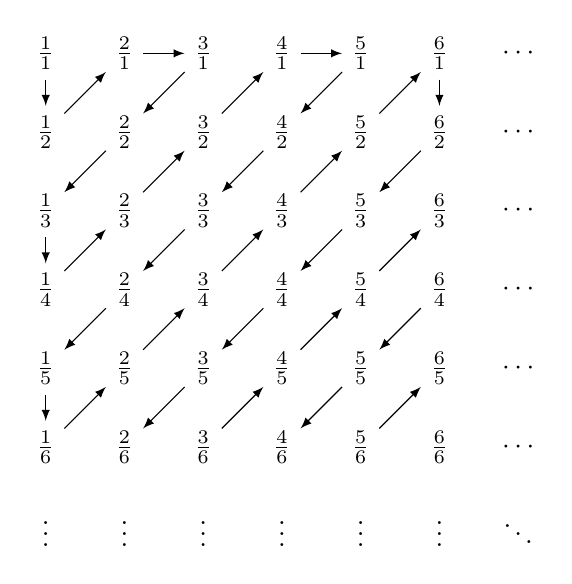
\begin{tikzpicture}[%
    >=latex
]
    \foreach\y in {1, 2, 3, 4, 5, 6}{%
        \foreach\x in {1, 2, 3, 4, 5, 6}{%
            \node (\x\y) at (\x, 7-\y) {$\frac{\x}{\y}$};
        }
    }
    \foreach\x in {1, 2, 3, 4, 5, 6}{%
        \node at (7, \x) {$\cdots$};
        \node at (\x, 0) {$\vdots$};
    }
    \node at (7, 0) {$\ddots$};
    \draw[->] (11) to (12);
    \draw[->] (12) to (21);
    \draw[->] (21) to (31);
    \draw[->] (31) to (22);
    \draw[->] (22) to (13);
    \draw[->] (13) to (14);
    \draw[->] (14) to (23);
    \draw[->] (23) to (32);
    \draw[->] (32) to (41);
    \draw[->] (41) to (51);
    \draw[->] (51) to (42);
    \draw[->] (42) to (33);
    \draw[->] (33) to (24);
    \draw[->] (24) to (15);
    \draw[->] (15) to (16);
    \draw[->] (16) to (25);
    \draw[->] (25) to (34);
    \draw[->] (34) to (43);
    \draw[->] (43) to (52);
    \draw[->] (52) to (61);
    \draw[->] (61) to (62);
    \draw[->] (62) to (53);
    \draw[->] (53) to (44);
    \draw[->] (44) to (35);
    \draw[->] (35) to (26);
    \draw[->] (36) to (45);
    \draw[->] (45) to (54);
    \draw[->] (54) to (63);
    \draw[->] (64) to (55);
    \draw[->] (55) to (46);
    \draw[->] (56) to (65);
\end{tikzpicture}
\end{document}
